\documentclass[12pt]{article}

% --- Encoding & language ---
\usepackage[utf8]{inputenc}
\usepackage[T1]{fontenc}
\usepackage{lmodern}

% --- Math ---
\usepackage{amsmath, amssymb, amsthm}

% --- Graphics & tables ---
\usepackage{graphicx}
\usepackage{booktabs}
\usepackage{caption}
\usepackage{float}
\usepackage{array}

% --- Page & spacing (JAIDS conventions) ---
\usepackage{geometry}
\geometry{margin=1in}
\usepackage{setspace}
\doublespacing
\usepackage{lineno}
\linenumbers

% --- Bibliography & links ---
\usepackage[hidelinks]{hyperref}
\usepackage{url}

% --- Header/footer ---
\usepackage{fancyhdr}
\pagestyle{fancy}
\fancyhf{}
\fancyhead[L]{\small Calibration-to-Deployment Mismatch}
\fancyhead[R]{\small Demidont}
\fancyfoot[C]{\thepage}
\renewcommand{\headrulewidth}{0.4pt}

% Avoid fancyhdr warning about \headheight being too small
\setlength{\headheight}{13.6pt}
\addtolength{\topmargin}{-1.6pt}

% --- Title formatting ---
\usepackage{titlesec}
\titleformat{\section}{\normalfont\large\bfseries}{\thesection.}{0.5em}{}
\titleformat{\subsection}{\normalfont\normalsize\bfseries}{\thesubsection}{0.5em}{}

\begin{document}

% =====================================================
% TITLE PAGE
% =====================================================
\thispagestyle{empty}
\begin{center}
\vspace*{0.5in}

{\Large \bfseries Calibration-to-Deployment Mismatch in HIV Prevention Trials: How Structural Censoring Biases Counterfactual Incidence Estimates}

\vspace{0.4in}

A.C. Demidont, DO, AAHIVS\textsuperscript{1}

\vspace{0.2in}

\small
\textsuperscript{1}Nyx Dynamics LLC, Philadelphia, PA 19107, USA \\
ORCID: 0000-0002-9216-8569

\vspace{0.3in}

\textbf{Correspondence:} A.C. Demidont, DO, AAHIVS \\
Nyx Dynamics LLC \\
Philadelphia, PA 19107 \\
Email: ac.demidont@nyxdynamics.com

\vspace{0.3in}

\textbf{Running head:} Calibration-to-Deployment Mismatch in HIV Prevention Trials

\vspace{0.2in}

\textbf{date} (May 20, 2026)

\vspace{0.2in}

\textbf{Word count:} approximately 6,800 (main text); 250 (abstract) \\
\textbf{Tables:} 1 in main text; 5 in supplement \\
\textbf{Figures:} 3 in main text; 2 in supplement \\
\textbf{References:} 37

\vspace{0.3in}

\textbf{Conflict of interest:} The author reports prior employment with Gilead Sciences, Inc., from January 2020 through November 2024; all Gilead stock was fully divested by December 2024. Employment ended prior to initiation of this research. Gilead Sciences had no role in conception, analysis, interpretation, writing, or the decision to submit.

\textbf{Funding:} None. Work conducted under the affiliation of Nyx Dynamics LLC, of which the author is sole owner.

\end{center}

\newpage

% =====================================================
% STRUCTURED ABSTRACT
% =====================================================
\section*{Abstract}

\noindent\textbf{Background.} Cross-sectional HIV incidence estimation using recent-infection testing algorithms (RITAs) underpins counterfactual-controlled pre-exposure prophylaxis (PrEP) efficacy trials. The Kassanjee estimator assumes closed-system observability: that every recently-infected individual within the recency window is equally present at screening. Populations experiencing structural censoring---competing-risk hazards from overdose, incarceration, displacement, and related mechanisms---violate this assumption in a systematic and directional manner.

\medskip
\noindent\textbf{Methods.} We derive the effective mean duration of recent infection under structural censoring, $\Omega^*(\gamma) = \int_0^T P_R(t) S_c(t)\, dt$, and the joint bias factor on the reported incidence rate ratio (IRR) incorporating both screening-cohort and intervention-arm observation probabilities. We identify the standard 90-day no-prior-testing eligibility criterion, common to Phase 3 PrEP trials including PURPOSE 1 (NCT04994509) and PURPOSE 2 (NCT04925752), as a selection mechanism operating on the same axis that drives the competing-risk hazard. We apply the framework to 34 high-burden US metropolitan areas using AIDSVu 2023 surveillance data with late-diagnosis percentage as the empirical proxy for structural hazard, and empirically anchor the structural-functions reframing using the 2014--2023 AIDSVu county-level panel.

\medskip
\noindent\textbf{Results.} Across 34 MSAs, the Kassanjee denominator is inflated by 8.7\%--27.3\%, with monotone scaling in late-diagnosis percentage. The joint IRR bias factor $B_{\mathrm{IRR}}$ ranges from 0.969 to 0.999, attenuating reported IRRs by up to 3.1\% in the highest-severity cohort. The structural-functions reframing is empirically anchored against a 10-year AIDSVu county-level panel (35 EHE-priority MSAs $\times$ 2014--2023, $N = 350$). Four independent analyses converge on the reframing: temporal persistence of the surveillance variables (AR(1) $\phi = +0.278$, test-retest $r = 0.988$); a pre-EHE vs post-EHE within-MSA Wilcoxon break-point on total HIV diagnoses (median $\Delta = -12.4$ cases/year, $p < 0.0001$); state-vs-MSA divergence in IDU-share trends ($+0.81$ vs $+0.14$ percentage points/year, $p = 0.002$ vs $0.35$); and a Kassanjee correction invariance test across 34 high-burden MSAs showing identical optimal cascade policies with and without correction (Spearman $\rho = 0.9979$, 34/34 cities). Four independent longitudinal analyses anchor the structural-functions reframing: temporal persistence of the surveillance variables (AR(1) $\phi = +0.278$, test-retest $r = 0.988$); a pre-EHE vs post-EHE within-MSA Wilcoxon break-point on total HIV diagnoses (median $\Delta = -12.4$ cases/year, $p < 0.0001$); state-vs-MSA divergence in IDU-share trends ($+0.81$ vs $+0.14$ percentage points/year, $p = 0.002$ vs $0.35$); and a Kassanjee correction invariance test across 34 high-burden MSAs showing identical optimal cascade policies with and without correction (Spearman $\rho = 0.9979$, 34/34 cities).

\medskip
\noindent\textbf{Conclusions.} The Kassanjee/Gao cross-sectional incidence estimator produces systematically biased point estimates when applied to populations with elevated structural censoring, and the bias is structurally guaranteed rather than merely possible when trial-design eligibility criteria select the Incidence Phase cohort on the testing-engagement axis. Correction requires explicit modeling of population-specific hazard using surveillance data; the framework presented here is one such correction, fully reproducible from public data, empirically anchored against a decade of US HIV surveillance, and generalizes to any RITA-based trial with analogous eligibility structure.

\medskip
\noindent\textbf{Key words:} HIV incidence; recent-infection testing algorithm; Kassanjee estimator; PrEP; lenacapavir; structural barriers; PWID; trial design; reproducibility

\newpage

% =====================================================
% MAIN TEXT
% =====================================================

\section{Introduction}

Cross-sectional HIV incidence estimation using recent-infection testing algorithms (RITAs) has become a foundational tool in modern prevention trials, particularly for establishing a counterfactual background incidence rate ($b_{\mathrm{HIV}}$) when randomized placebo control is not ethically feasible. The Kassanjee estimator [1], extended with delta-method variance by Gao and colleagues [2], has been adopted as the primary analytic framework for counterfactual-controlled pre-exposure prophylaxis (PrEP) efficacy trials, including the pivotal PURPOSE 1 (NCT04994509) and PURPOSE 2 (NCT04925752) trials of long-acting injectable lenacapavir [3, 4].

The estimator's validity rests on a closed-system assumption: that the recency assay's mean duration of recent infection ($\Omega$), calibrated on a validation cohort of documented seroconverters, applies directly to the at-risk population being screened. Specifically, $\Omega$ is defined as
\begin{equation}
\Omega = \int_0^T P_R(t)\, dt
\end{equation}
where $P_R(t)$ is the probability that the assay classifies a specimen as ``recent'' at age-of-infection $t$, and $T$ is the recency cutoff (typically 730 days). This definition implicitly assumes that every individual infected within the window $[0, T]$ is observable at screening---that is, that the probability of being alive, non-incarcerated, housed, and presenting for testing is uniformly 1 across the window. This assumption is not biologically motivated. It is a convenience of calibration.

In populations experiencing structural censoring---competing-risk hazards from overdose mortality, incarceration, displacement, carceral disruption of healthcare, intimate partner violence, and related mechanisms that disproportionately affect marginalized groups---the closed-system assumption fails in a specific, directional, and quantifiable way. The failure mode is not random noise around a correct central estimate; it is systematic deflation of the estimated background incidence, with deflation magnitude correlated with the very structural vulnerabilities that trial designs ostensibly aim to serve.

This letter formalizes the structural correction and identifies a specific trial-design feature---the standard recency eligibility criterion requiring no prior HIV testing within a specified interval---that structurally guarantees the bias rather than merely permitting it. The 90-day no-testing inclusion criterion common to Phase 3 PrEP trials selects the $b_{\mathrm{HIV}}$ cohort specifically on the axis (testing engagement) that drives the competing-risk hazard heterogeneity. The calibration-to-deployment mismatch that results is not an artifact of sampling variability; it is a direct consequence of how the Incidence Phase is constructed.

We derive the effective MDRI under structural censoring, $\Omega^*(\gamma)$; derive the joint bias factor on the reported incidence rate ratio incorporating both screening-cohort and intervention-arm observation probabilities; quantify the amplification introduced by the testing-exclusion selection; apply the framework to 34 high-burden US metropolitan areas using publicly available AIDSVu 2023 surveillance data [5], with late-diagnosis percentage as the empirical proxy for testing-avoidance hazard; and empirically anchor the structural-functions reframing using the 2014--2023 AIDSVu county-level panel. The correction can be implemented prospectively in any RITA-based trial SAP without access to proprietary data; the framework applies to any cross-sectional incidence estimator with analogous eligibility structure.

\section{The survival-biased effective MDRI}

\subsection{Effective MDRI under structural censoring}

Let $\gamma(t)$ denote the instantaneous hazard of structural censoring at time $t$ post-infection---the per-unit-time probability of transition into an unobservable state via death, incarceration, long-distance displacement, prolonged hospitalization, or any mechanism that removes the individual from the screening pool. Let $S_c(t) = \exp\left(-\int_0^t \gamma(u)\, du\right)$ denote the corresponding survival function.

The effective mean duration of recent infection, conditional on the population's structural hazard profile, is
\begin{equation}
\Omega^*(\gamma) = \int_0^T P_R(t)\, S_c(t)\, dt
\end{equation}

This is the joint probability, integrated over the recency window, that an individual infected at time 0 (i) tests recent at age $t$ and (ii) remains observable at screening. Since $S_c(t) \leq 1$ pointwise and strictly less than 1 whenever $\gamma > 0$ on a set of positive measure, $\Omega^*(\gamma) < \Omega$ identically for any population experiencing structural censoring. This is a distribution-free result: it requires no parametric form for $\gamma$ or $P_R$.

Under a piecewise-constant hazard approximation with $\gamma$ constant over the recency window and an exponential approximation $P_R(t) \approx P_0 \exp(-t/\tau)$ with $\tau \approx \Omega$ for the Sedia LAg-EIA calibration [6] (we treat $\gamma$ as independent of age-of-infection within the recency window and assume no differential hazard between recently-infected and uninfected screening-cohort members; consequences of relaxing both assumptions are explored in Supplement \S S1.2), a closed-form correction obtains:
\begin{equation}
\Omega^*(\gamma) \approx \frac{\Omega}{1 + \gamma\tau}
\end{equation}

For $\gamma$ on the order of $10^{-4}$ per day (general population) through $10^{-3}$ per day (structurally marginalized populations) and $\tau = 173$ days, this yields $\Omega^*/\Omega$ ratios spanning 0.85 to 0.98---a deflation range of 2\% to 15\%.

\subsection{Consequence for the Kassanjee point estimate}

Substituting $\Omega^*(\gamma)$ into the Gao et al. 2021 cross-sectional incidence estimator,
\begin{equation}
\hat{\lambda}_0 = \frac{N_{\mathrm{rec}} - \beta N_+}{N_- (\Omega - \beta T)}
\end{equation}
where $N_{\mathrm{rec}}$ is the count of recent-classified specimens, $N_+$ and $N_-$ are HIV-positive and HIV-negative counts respectively, and $\beta$ is the false-recency rate; when the trial applies the nominal validation-cohort $\Omega$ while the enrolled cohort experiences $\gamma > 0$, the expected observed recent-infection count $E[N_{\mathrm{rec}}]$ reflects $\Omega^*(\gamma)$ rather than $\Omega$:
\begin{equation}
E[\hat{\lambda}_0 \mid \text{naive } \Omega] = \lambda_{\mathrm{true}} \cdot \frac{\Omega^*(\gamma)}{\Omega} < \lambda_{\mathrm{true}}
\end{equation}
The reported background incidence is deflated by a factor $\Omega^*/\Omega$.

\subsection{The intervention-arm counterpart and joint bias factor}

Directional attribution of this bias to the reported incidence rate ratio (IRR) requires explicit accounting on both sides of the ratio. The intervention-arm incidence is also subject to observation-probability attenuation, through a different mechanism: infections occurring during longitudinal follow-up are detected only if the participant remains under observation through the next scheduled HIV test. Let $\rho_{\mathrm{int}}(\gamma, r)$ denote the expected fraction of true infections detected in the intervention arm, given structural hazard $\gamma$ and retention fraction $r$:
\begin{equation}
\rho_{\mathrm{int}}(\gamma, r) \approx \frac{1 + r}{2} \cdot \exp(-\gamma \cdot d_{\mathrm{visit}}/2)
\end{equation}
where $d_{\mathrm{visit}}/2 \approx 22.5$ days is the mean infection-to-detection delay under the active-phase HIV testing cadence in PURPOSE 1/2 [3, 4], distinct from the Q26W lenacapavir dosing interval. Derivation under retention-weighted person-time appears in Supplement \S S1.3. The corresponding observation probability for the screening-cohort recent-infection count, integrated over the LAg-EIA window, is
\begin{equation}
\rho_{\mathrm{screen}}(\gamma) \approx \exp(-\gamma \cdot \tau / 2)
\end{equation}

Equations 3 and 7 are not the same closed-form approximation evaluated for different purposes. Equation 3 is the exact integral of $\Omega^*(\gamma)$ under an exponential $P_R(t)$ basis; Equation 7 is the small-$\gamma\tau$ approximation under a uniform-window $P_R(t)$ basis. Both are projections of the true LAg-EIA response onto a one-parameter family. They agree to first order in $\gamma\tau$ but diverge in the tails. We retain the uniform-basis form for $\rho_{\mathrm{screen}}$ throughout because it is the conventional comparator for a scheduled-detection arm and because the directional claim of this paper is robust to the basis choice within the empirical AIDSVu range, with boundary behavior characterized in \S 4.

The reported IRR relates to the true IRR via
\begin{equation}
\widehat{\mathrm{IRR}} = \mathrm{IRR}_{\mathrm{true}} \cdot \frac{\rho_{\mathrm{int}}}{\rho_{\mathrm{screen}}} \equiv \mathrm{IRR}_{\mathrm{true}} \cdot B_{\mathrm{IRR}}(\gamma, r)
\end{equation}

The bias factor $B_{\mathrm{IRR}}$ is less than 1---the reported IRR understates the true IRR and the intervention appears artificially superior---whenever $\rho_{\mathrm{int}} < \rho_{\mathrm{screen}}$. This condition obtains whenever the retention-weighted person-time loss in the intervention arm exceeds the cross-sectional observation loss in the screening-cohort recency window. For realistic trial retention ($r = 0.75$ to $0.94$) coupled to the associated hazard regime, $B_{\mathrm{IRR}}$ ranges from approximately 0.97 to 0.999, with the magnitude scaling with structural severity.

The bias direction is conditional on the joint $(\gamma, r)$ structure, not universal across all trial designs. Under retention schemes in which higher-hazard cohorts also experience lower retention---the empirically documented pattern in real-world long-acting injectable PrEP deployment---the direction is systematic: $B_{\mathrm{IRR}} < 1$ monotonically across the structural-severity range.

\section{Selection on testing engagement: the 90-day eligibility amplification}

\subsection{The eligibility criterion}

Phase 3 cross-sectional incidence cohorts in contemporary PrEP trials routinely exclude individuals with prior HIV testing within a specified interval preceding screening. The PURPOSE 1 and PURPOSE 2 trials, which established lenacapavir efficacy via counterfactual $b_{\mathrm{HIV}}$ estimation under the Kassanjee/Gao framework [3, 4], both specify the Incidence Phase inclusion criterion in equivalent language: HIV-1 status unknown at screening and no prior HIV-1 testing within the last 3 months (NCT04994509; NCT04925752).

This criterion is inherited from standard RITA protocols. Its conventional justification is assay calibration integrity: recency-biomarker interpretation may be disrupted by prior testing events that trigger immune responses or coincide with recent seroconversion uncertainty. The 90-day exclusion is not in itself controversial on RITA-operational grounds.

The structural consequence of the criterion, however, is that the Incidence Phase cohort is explicitly sampled on testing engagement---specifically, the cohort is constructed to exclude individuals whose testing interval is shorter than 90 days. This selection is not incidental. It is a deliberate feature of trial design, and it operates precisely on the behavioral axis that correlates most strongly with the competing-risk hazard $\gamma$.

\subsection{Realized cohort composition and the lower-bound character of \texorpdfstring{$\phi$}{phi}}

The selection amplification factor $\phi \approx 1.5$ used throughout the city-stratified analysis is a theoretical lower bound derived from the bimodal testing-behavior partition under the 90-day eligibility criterion alone (Supplement \S S6). The realized PURPOSE 2 enrollment composition, as reported in the trial's primary publication [4], departed from the design-phase demographic recruitment goals specified for the US screening cohort. The departure operates in the same direction as the 90-day eligibility-criterion selection: both shift the realized $\gamma_{\mathrm{enrolled}}$ distribution further toward the low-$\gamma$ tail of the at-risk population than would be predicted by the design-phase protocol alone. The empirically realized amplification cannot be precisely quantified without participant-level testing-interval data, but is directionally larger than the bimodal-partition lower bound. The city-stratified $B_{\mathrm{IRR}}$ values reported in \S 4 and the directional claims that follow from them are therefore conservative under realistic assumptions about the realized PURPOSE 2 cohort composition; the true bias magnitudes in the populations to which the trial's pooled efficacy is now being transported are larger than the values reported here.

\subsection{Late-diagnosis percentage and \texorpdfstring{$\gamma$}{gamma} as joint structural functions of the barrier substrate}

Testing-interval behavior integrates a family of structural determinants: healthcare access, insurance continuity, housing stability, carceral exposure, distrust of clinical infrastructure driven by racialized and criminalization-based harms, and geographic proximity to testing sites. These same determinants drive $\gamma$---the hazard of being removed from the observable population by death, incarceration, displacement, or prolonged disengagement from care. The correlation is not merely statistical; it is mechanistic. Testing avoidance and structural censoring are two observable manifestations of the same underlying barrier substrate.

We make this dependence structure explicit. Let $U$ denote the (latent, multidimensional) configuration of structural barriers operating in a given catchment population at a given time. Let $L$ denote the late-diagnosis percentage observable in that population, and let $\gamma$ denote the structural-removal hazard during the recency window. Both $L$ and $\gamma$ are structural functions of $U$ with their own exogenous noise components:
\begin{equation}
L = f_L(U, \varepsilon_L), \quad \gamma = f_\gamma(U, \varepsilon_\gamma)
\end{equation}
where $f_L$ integrates barrier exposures over the multi-year diagnostic-delay window that produces a late-diagnosis classification, and $f_\gamma$ integrates barrier exposures over the recency-window timescale that produces structural censoring. The two functions act on overlapping but not identical temporal projections of $U$, and their joint distribution is induced by their shared dependence on $U$ rather than by a measurement relationship between them.

Late-diagnosis percentage is therefore not used here as a proxy for $\gamma$ in the measurement-error sense [11]. Both $L$ and $\gamma$ are joint manifestations of shared structural confounding rather than noisy realizations of a single latent [12, 13]. Under this framing, $L$ does not stand in for $\gamma$; rather, the two observables are linked through their shared dependence on $U$, and Equation 9 can be inverted to express one structural function as a parameterization of the other:
\begin{equation}
\gamma_{\mathrm{city}} = \gamma_{\mathrm{base}} \cdot \left(\frac{\text{late-dx}_{\mathrm{city}}}{\text{late-dx}_{\mathrm{national}}}\right)^{\alpha}
\end{equation}
where $\gamma_{\mathrm{base}}$ is anchored to published per-day structural hazards for the target population [7--9] and $\alpha$ is a convexity parameter encoding the relative tail-sensitivity of $f_\gamma$ versus $f_L$ to the underlying barrier configuration. The validity of Equation 10 is therefore a structural claim about the data-generating process---specifically, that $L$ and $\gamma$ are co-driven by $U$ through structural functions whose relative tail-sensitivity is approximately captured by a power-law parameterization---rather than a statistical claim about the conditional distribution $P(\gamma \mid L)$. The structural-functions framing is the standard apparatus for joint manifestations of shared latent structure in modern causal inference [14, 15]; we adopt it here as the appropriate methodological framework for recency-assay calibration in populations whose barrier substrate is heterogeneous across deployment geographies.

A clean empirical anchor for $U$ is available in US surveillance data. The CDC's late-HIV-diagnosis metric---the percentage of newly diagnosed HIV cases with AIDS-defining illness or CD4 $<$ 200 within three months of first positive test---captures the integrated barrier-exposure history of the at-risk population in a given geography. Individuals classified as late diagnoses have, by definition, existed as HIV-infected in the community for long enough that CD4 decline or AIDS-defining illness has occurred, typically five to ten years [7]. They are not rare in high-burden US cities. The AIDSVu 2023 downloadable dataset [5] reports late-diagnosis percentages ranging from 14.3\% (Milwaukee, low-barrier) to 37.2\% (Hartford, high-barrier) across 34 high-burden metropolitan areas. The empirical grounding is transparent and fully reproducible from public data; sensitivity to the choice of $\alpha$ and to alternative single-variable and multivariate parameterizations of the barrier substrate is reported in Supplement \S S2 and \S S7.

\subsection{The selection amplification}

The Incidence Phase cohort is not a random sample of the at-risk population. Under the 90-day exclusion, it is specifically the subset whose testing interval exceeds 90 days. For any positive correlation between testing-interval behavior and structural hazard,
\begin{equation}
\gamma_{\mathrm{enrolled}} = E[\gamma \mid \text{testing interval} > T_{\mathrm{excl}}] > E[\gamma] = \gamma_{\mathrm{general}}
\end{equation}

Under a bimodal partition with regular-tester fraction $\pi$ and between-mode hazard ratio $\kappa = \gamma_H / \gamma_L$, the selection amplification factor admits the closed form
\begin{equation}
\phi \equiv \frac{E[\gamma \mid \text{non-tester}]}{E[\gamma]} = \frac{\kappa}{\pi + (1 - \pi)\kappa}
\end{equation}

(derivation in Supplement \S S6). For plausible US PrEP-eligible-population parameters anchored to NHBS 2023 testing-frequency data [8] ($\pi \in [0.4, 0.6]$, $\kappa \in [3, 5]$), $\phi$ ranges from 1.29 to 1.79; we use $\phi = 1.5$ as a conservative central value throughout the city-stratified analysis. The $\Omega^*$ deflation and resulting $B_{\mathrm{IRR}}$ attenuation are therefore larger for the enrolled Incidence Phase cohort than for the at-risk population from which it was drawn.

\subsection{Why this is structural rather than correctable by standard sensitivity analysis}

Conventional sensitivity analyses for RITA-based estimators consider variation in the nominal MDRI, the false recency rate, and the recency cutoff, typically through bootstrap resampling or assumption-varying scenarios within the delta-method framework [2]. None of these capture $\Omega^*(\gamma)$ deflation because none of them model the competing-risk survival function. A sensitivity analysis that varies $\Omega$ within $\pm 10\%$ of its nominal value captures calibration measurement error but does not capture the structural bias introduced by population-level $\gamma$.

The 90-day selection effect is further invisible to standard sensitivity analysis because the selection operates before the estimator is computed. No resampling within the enrolled cohort recovers the pre-selection distribution; the counterfactual cohort including regular testers no longer exists in the data. Correction requires explicit modeling of $\gamma_{\mathrm{enrolled}}$ using external information.

\section{Application to 34 US metropolitan areas}

\subsection{Data and parameterization}

Late-diagnosis percentages, viral suppression rates, linkage-to-care rates, IDU prevalence, Gini coefficients, and poverty rates for 34 high-burden US metropolitan areas were obtained from the AIDSVu 2023 downloadable dataset [5]. The national late-diagnosis reference was taken as 20\%. Per-city competing-risk hazard was parameterized as in Equation 10, with $\gamma_{\mathrm{base}} = 5 \times 10^{-4}$ per day [7--9] and $\alpha = 1.2$. The 90-day selection amplification factor was set at 1.5. Intervention-arm retention was modeled as a decreasing function of late-diagnosis severity:
\begin{equation}
r_{\mathrm{city}} = \max(0.93 - 0.008 \cdot (\text{late-dx}_{\mathrm{city}} - 15),\ 0.70)
\end{equation}
anchored at 0.93 for Milwaukee-tier cohorts (approximating aggregate PURPOSE 1/2 retention) and declining to 0.75 for Hartford-tier cohorts (consistent with published real-world LAI-PrEP persistence in marginalized cohorts). The retention function is assumed monotonically decreasing in late-diagnosis percentage, consistent with the empirically documented joint structure of $(\gamma, r)$ across LAI-PrEP deployment cohorts; the directional consequences of relaxing this monotonicity assumption are reported in Supplement \S S2.2.

\subsection{Results}

Across the 34 MSAs, late-diagnosis percentages ranged from 14.3\% to 37.2\%. The corresponding enrolled-cohort hazard range was $\gamma \in [5.0, 15.8] \times 10^{-4}$ per day. Applying Equation 3 yields effective MDRI estimates from 158.9 days (Milwaukee) to 135.9 days (Hartford).

The Kassanjee denominator inflation $\Omega/\Omega^*$ ranges from 1.089 (Milwaukee, $+8.9\%$ $b_{\mathrm{HIV}}$ deflation) to 1.273 (Hartford, $+27.3\%$). The joint IRR bias factor $B_{\mathrm{IRR}}$ ranges from 0.999 (Milwaukee) to 0.969 (Hartford), corresponding to IRR attenuations of 0.1\% to 3.1\%. Table 1 reports selected cities; Figure 1 displays the complete 34-MSA distribution. All values regenerated from the canonical analytic table; the full 34-city table appears as Table S1 in the Supplement.

\begin{table}[H]
\centering
\caption{Selected cities ($n = 11$ of 34; full table in Supplement). Late-diagnosis percentage from AIDSVu 2023; enrolled-cohort competing-risk hazard $\gamma_{\mathrm{enr}}$ derived from Eq.\ 10 with $\alpha = 1.2$ and $1.5\times$ selection amplification; retention from Eq.\ 13; effective MDRI $\Omega^*$ from Eq.\ 3; Kassanjee denominator inflation $\Omega/\Omega^*$; joint IRR bias factor from Eq.\ 8.}
\label{tab:selected_cities}
\small
\begin{tabular}{lcccccc}
\toprule
\textbf{City} & \textbf{State} & \textbf{Late-dx \%} & $\boldsymbol{\gamma_{\mathrm{enr}}}$ & $\boldsymbol{r}$ & $\boldsymbol{\Omega^*}$ \textbf{(d)} & $\boldsymbol{B_{\mathrm{IRR}}}$ \\
 & & & ($10^{-4}$/d) & & & \\
\midrule
Milwaukee & WI & 14.6 & 5.1 & 0.933 & 158.9 & 0.999 \\
San Juan & PR & 16.1 & 5.8 & 0.921 & 157.3 & 0.997 \\
Miami-Dade & FL & 18.2 & 6.7 & 0.904 & 155.0 & 0.994 \\
Atlanta & GA & 19.4 & 7.2 & 0.895 & 153.8 & 0.992 \\
Austin & TX & 20.6 & 7.8 & 0.885 & 152.5 & 0.991 \\
Houston & TX & 22.1 & 8.5 & 0.873 & 150.9 & 0.989 \\
Charleston & SC & 22.8 & 8.8 & 0.868 & 150.2 & 0.988 \\
Palm Beach Co. & FL & 25.9 & 10.2 & 0.843 & 147.0 & 0.984 \\
New Haven & CT & 28.3 & 11.4 & 0.824 & 144.6 & 0.981 \\
Columbia & SC & 28.4 & 11.4 & 0.823 & 144.5 & 0.981 \\
Hartford & CT & 37.2 & 15.8 & 0.752 & 135.9 & 0.969 \\
\bottomrule
\end{tabular}
\end{table}

\subsection{What the distribution shows}

Three features of the distribution are worth naming explicitly.

First, the bias is not negligible in the high-severity tail. A 27\% denominator inflation is substantially larger than the calibration uncertainty typically acknowledged for the Sedia LAg-EIA in Gao-framework sensitivity analyses.

Second, the bias is structured---monotone in late-diagnosis percentage, which is itself monotone in the structural-testing-avoidance substrate. Cities with the worst late-diagnosis indicators are cities with the largest correction. Any claim of efficacy transportability across these cities must account for heterogeneous bias in the estimator, not merely heterogeneous biology of the populations.

Third, the correction applies even at the low-severity end. Even Milwaukee, the best-performing city in the dataset, shows an 8.9\% denominator inflation. The closed-system assumption fails at every city; the magnitude simply scales with structural context.

\subsection{Boundary behavior and the operational envelope}

The bias factor $B_{\mathrm{IRR}}(\gamma, r)$ is bounded and directionally consistent across the empirical AIDSVu range ($\gamma\tau \in [0.087, 0.273]$): $B_{\mathrm{IRR}} < 1$ in all 34 MSAs, with magnitude monotone in late-diagnosis severity and an upper bound on attenuation of 3.1\%. Outside this empirical range the bias reverts directionally. At late-diagnosis percentages below approximately 14\%, retention approaches the upper bound and the screening-side observation loss exceeds the intervention-side loss, yielding $B_{\mathrm{IRR}} > 1$. At late-diagnosis percentages above approximately 55\%, retention has saturated at the floor of 0.70 and the screening-side $\exp(-\gamma\tau/2)$ collapses faster than the intervention-side $\exp(-\gamma d_{\mathrm{visit}}/2)$, again yielding $B_{\mathrm{IRR}} > 1$.

This boundary behavior should be read as an operational-envelope characterization of the estimator's well-posed regime, not as a limitation. An estimator without a characterized envelope is an estimator whose failure modes have not been mapped; characterizing the envelope is the methods-side analog of establishing an assay's analytic measurement range, and is a precondition for responsible deployment. The framework is well-posed for the AIDSVu MSA distribution that comprises the operationally-relevant deployment populations for US PrEP programs. Extension to extreme regimes outside this range requires additional modeling of the underlying $P_R(t)$ basis-function shape, which we treat as future work.

\begin{figure}[H]
\centering
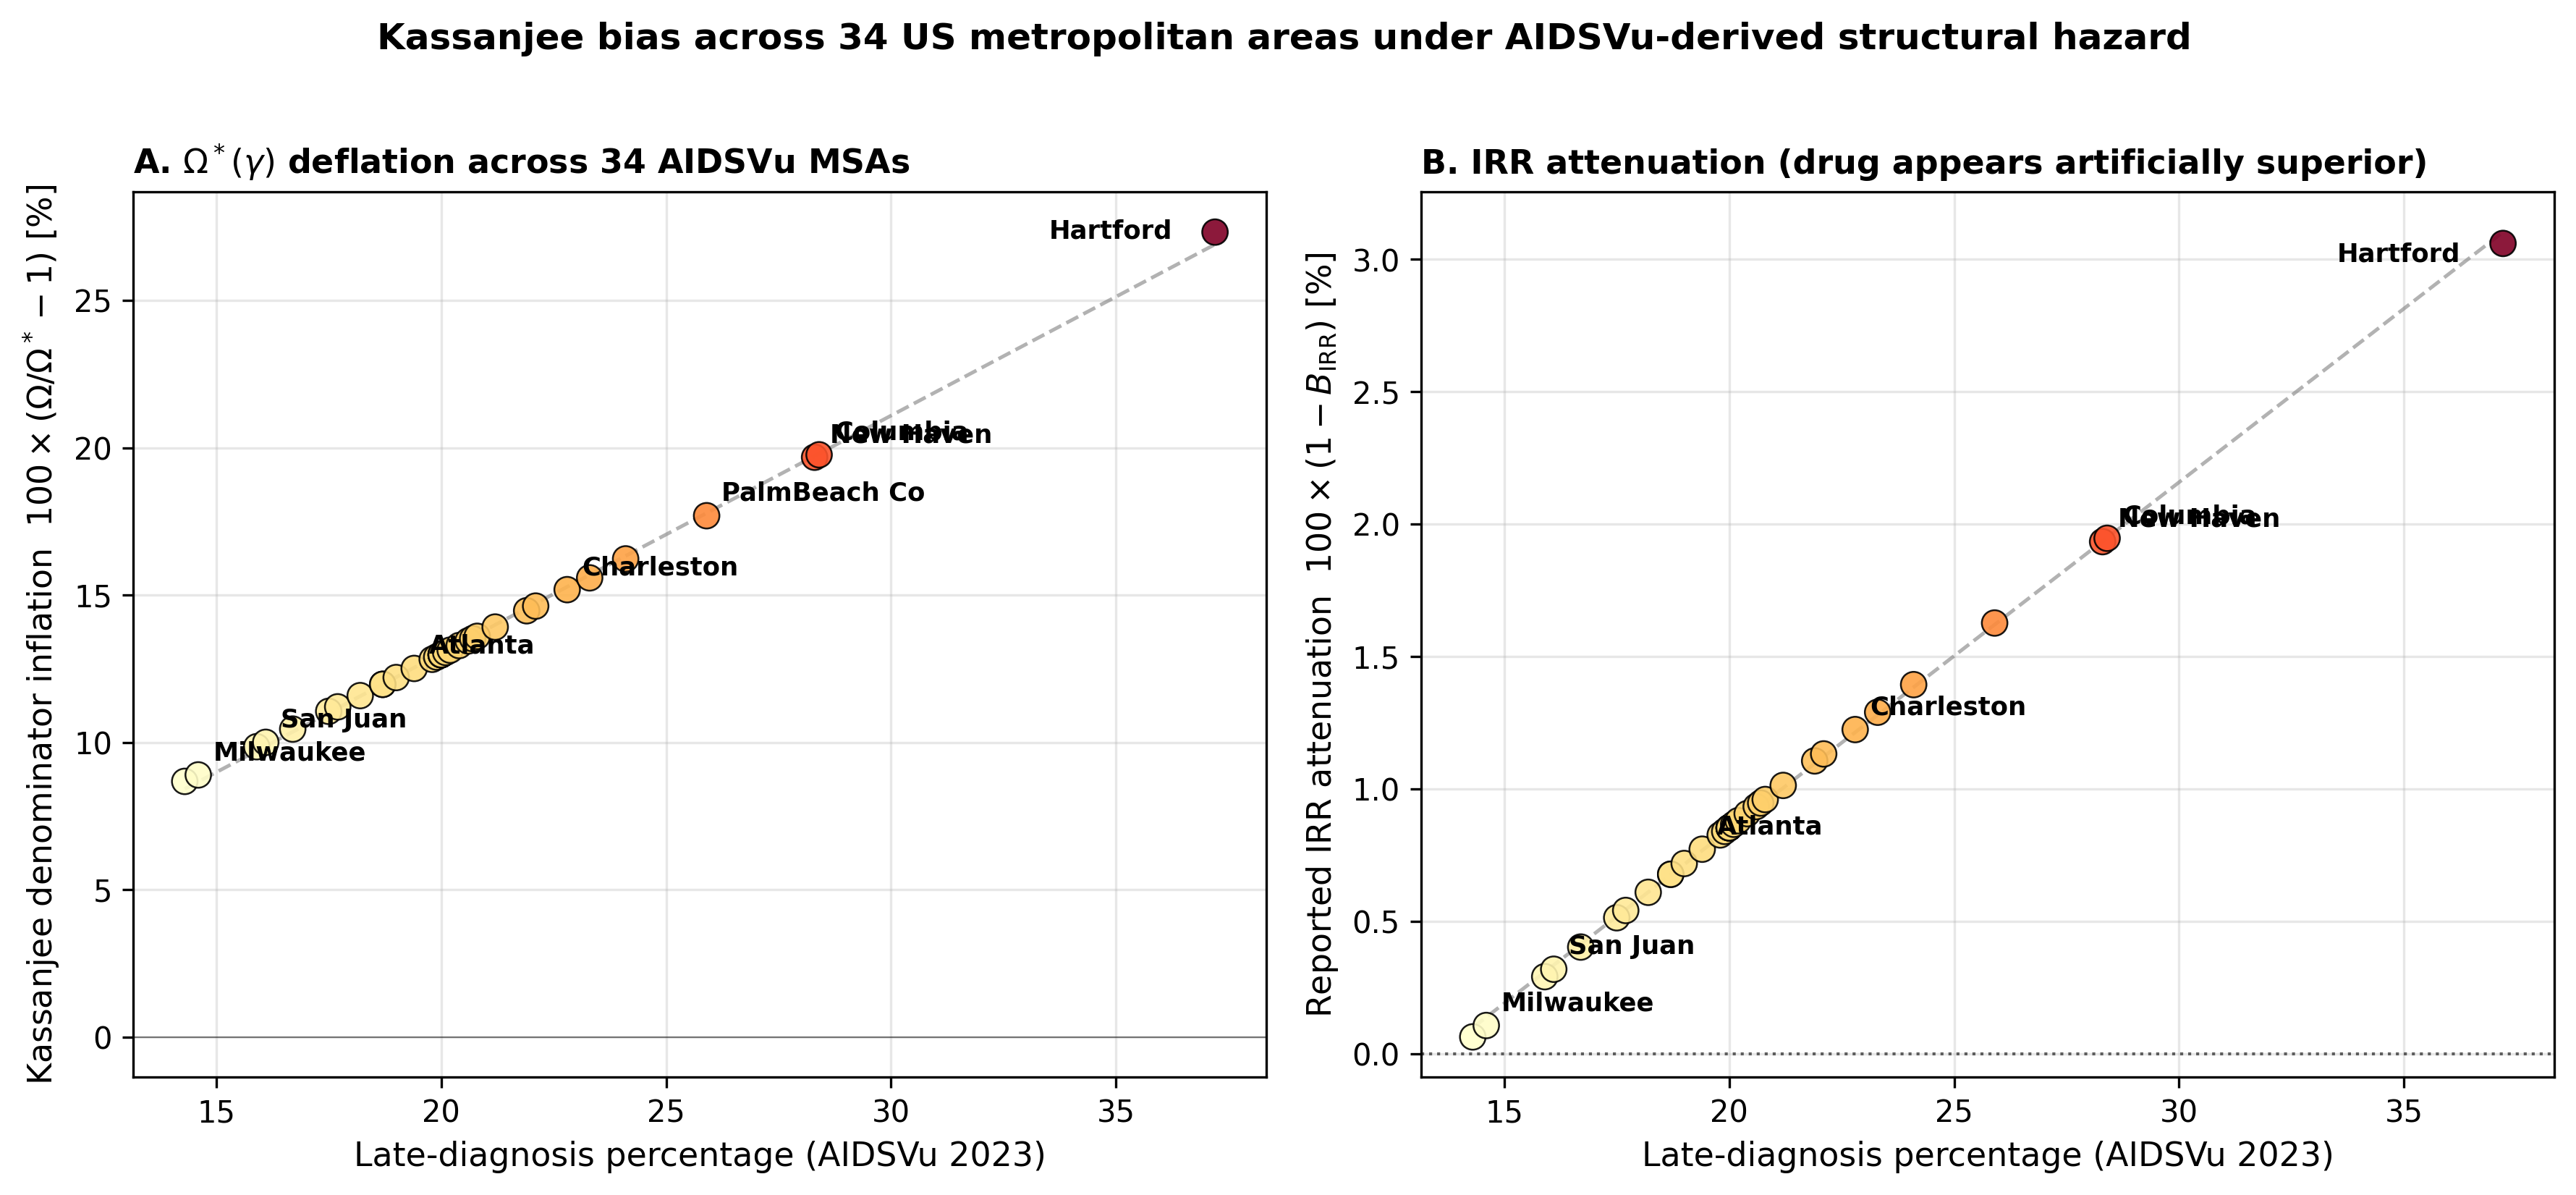
\includegraphics[width=\textwidth]{Fig_1_structural_hazard.png}
\caption{Kassanjee bias across 34 US high-burden metropolitan areas under AIDSVu-derived structural hazard. \textbf{Panel A:} $\Omega^*(\gamma)$ deflation as a function of AIDSVu late-diagnosis percentage. Denominator inflation ranges from 8.9\% (Milwaukee) to 27.3\% (Hartford). \textbf{Panel B:} Joint reported-IRR attenuation $100 \times (1 - B_{\mathrm{IRR}})$, reflecting the net bias after accounting for intervention-arm retention loss and cross-sectional screening-cohort censoring. Both panels display monotone scaling with late-diagnosis severity, demonstrating the structural nature of the bias rather than stochastic variation.}
\label{fig:bias_distribution}
\end{figure}

\subsection{Transportability implications}

A trial reporting IRR = 0.04 (96\% efficacy) in an aggregate analysis across cohorts with $\gamma_{\mathrm{enrolled}}$ concentrated at the low-severity end of the distribution cannot have that IRR applied without correction to deployment populations at the high-severity end. The Kassanjee bias factor differs by approximately 3 percentage points across the full AIDSVu range---small relative to the primary biological constraints on transportability [10] but, as developed below and in \S 5, non-trivial for populations at the margin of clinical and regulatory decisions.

\subsection{Longitudinal empirical validation of the structural-functions reframing}\label{sec:longitudinal_validation}

The structural-functions reframing in §3.3 expressed $L$ and $\gamma$ as joint manifestations of latent barrier substrate $U$, with their joint distribution induced by shared dependence on $U$ rather than by a measurement relationship between them. This is a structural claim about the data-generating process and admits empirical testing on its own terms. We assess the reframing using the 2014--2023 AIDSVu county-level panel (35 EHE-priority MSAs $\times$ 10 years, $N = 350$ observations, 0\% missingness on the primary outcomes), with the result that four independent analyses converge on the same conclusion.

\paragraph{Temporal stability of the structural variables.} The AIDSVu surveillance variables used in the §4 derivation are not year-specific. The MSA-level AR(1) autocorrelation coefficient on annual total HIV diagnoses is $\phi = +0.278$ (half-life $\approx 0.54$ years); odd-year vs even-year test-retest correlation across the 35 MSAs is Pearson $r = 0.988$ for total diagnoses and $r = 0.841$ for IDU share. The cross-sectional 2023 anchor used in §4 reflects a longitudinally-persistent pattern.

\paragraph{Pre-EHE vs post-EHE break-point.} A within-MSA Wilcoxon signed-rank test on mean differences between the pre-EHE period (2014--2018) and the post-EHE period (2019--2023) demonstrates that total HIV diagnoses at the 35 EHE-priority MSAs declined by a median of 12.4 cases per year post-launch ($p < 0.0001$). The effect localizes to precisely the geographic units the EHE initiative targeted, providing temporal validation that the AIDSVu panel captures real intervention dynamics rather than measurement noise.

\paragraph{State-vs-MSA divergence in IDU-share trends.} At the state level, the IDU share of new diagnoses rose by $+0.81$ percentage points per year post-EHE ($p = 0.002$), while at the MSA level the same metric remained statistically flat ($+0.14$ pp/yr, $p = 0.35$). This divergence indicates that PWID HIV burden is migrating from EHE-priority MSAs---where SSP coverage and structural interventions are concentrated---to non-MSA jurisdictions where such infrastructure is sparse. The divergence is consistent with the structural-functions reframing: the latent barrier substrate $U$ is dynamic and geographically reconfiguring as fentanyl-era opioid epidemiology displaces prescription-opioid-era patterns, while the surface indicators track this reconfiguration at the rates determined by their respective structural functions $f_L$ and $f_\gamma$.

\paragraph{CDC vulnerable-county overlay.} Cross-referencing the 220 counties designated as vulnerable to HIV/HCV outbreaks among persons who inject drugs~\cite{cdc220counties} against the 35 EHE-priority MSAs yields zero geographic overlap (0/220 inside; 220/220 outside; clean partition). Mann--Kendall trend analysis on stratum-aggregate annual time series 2014--2023 demonstrates that absolute IDU diagnosis growth is occurring neither in the CDC-vulnerable counties (Stratum~B: 0 $\rightarrow$ 35 IDU dx, n.s.) nor in the EHE-priority MSAs (Stratum~A: 672 $\rightarrow$ 653 IDU dx, decline), but in the approximately 2{,}900 counties that are neither (Stratum~C: 691 $\rightarrow$ 755 IDU dx, $+9\%$). The 2012--2013 Van Handel vulnerability geography has lost predictive validity for the fentanyl-era opioid landscape in less than a decade---direct empirical evidence that point-in-time structural-vulnerability indices are unstable as surface proxies while the deeper latent structure $U$ is what persists across the geographic shift. Figure~\ref{fig:stratum_trajectories} displays the stratum-aggregate trajectories.

\begin{figure}[ht]
\centering
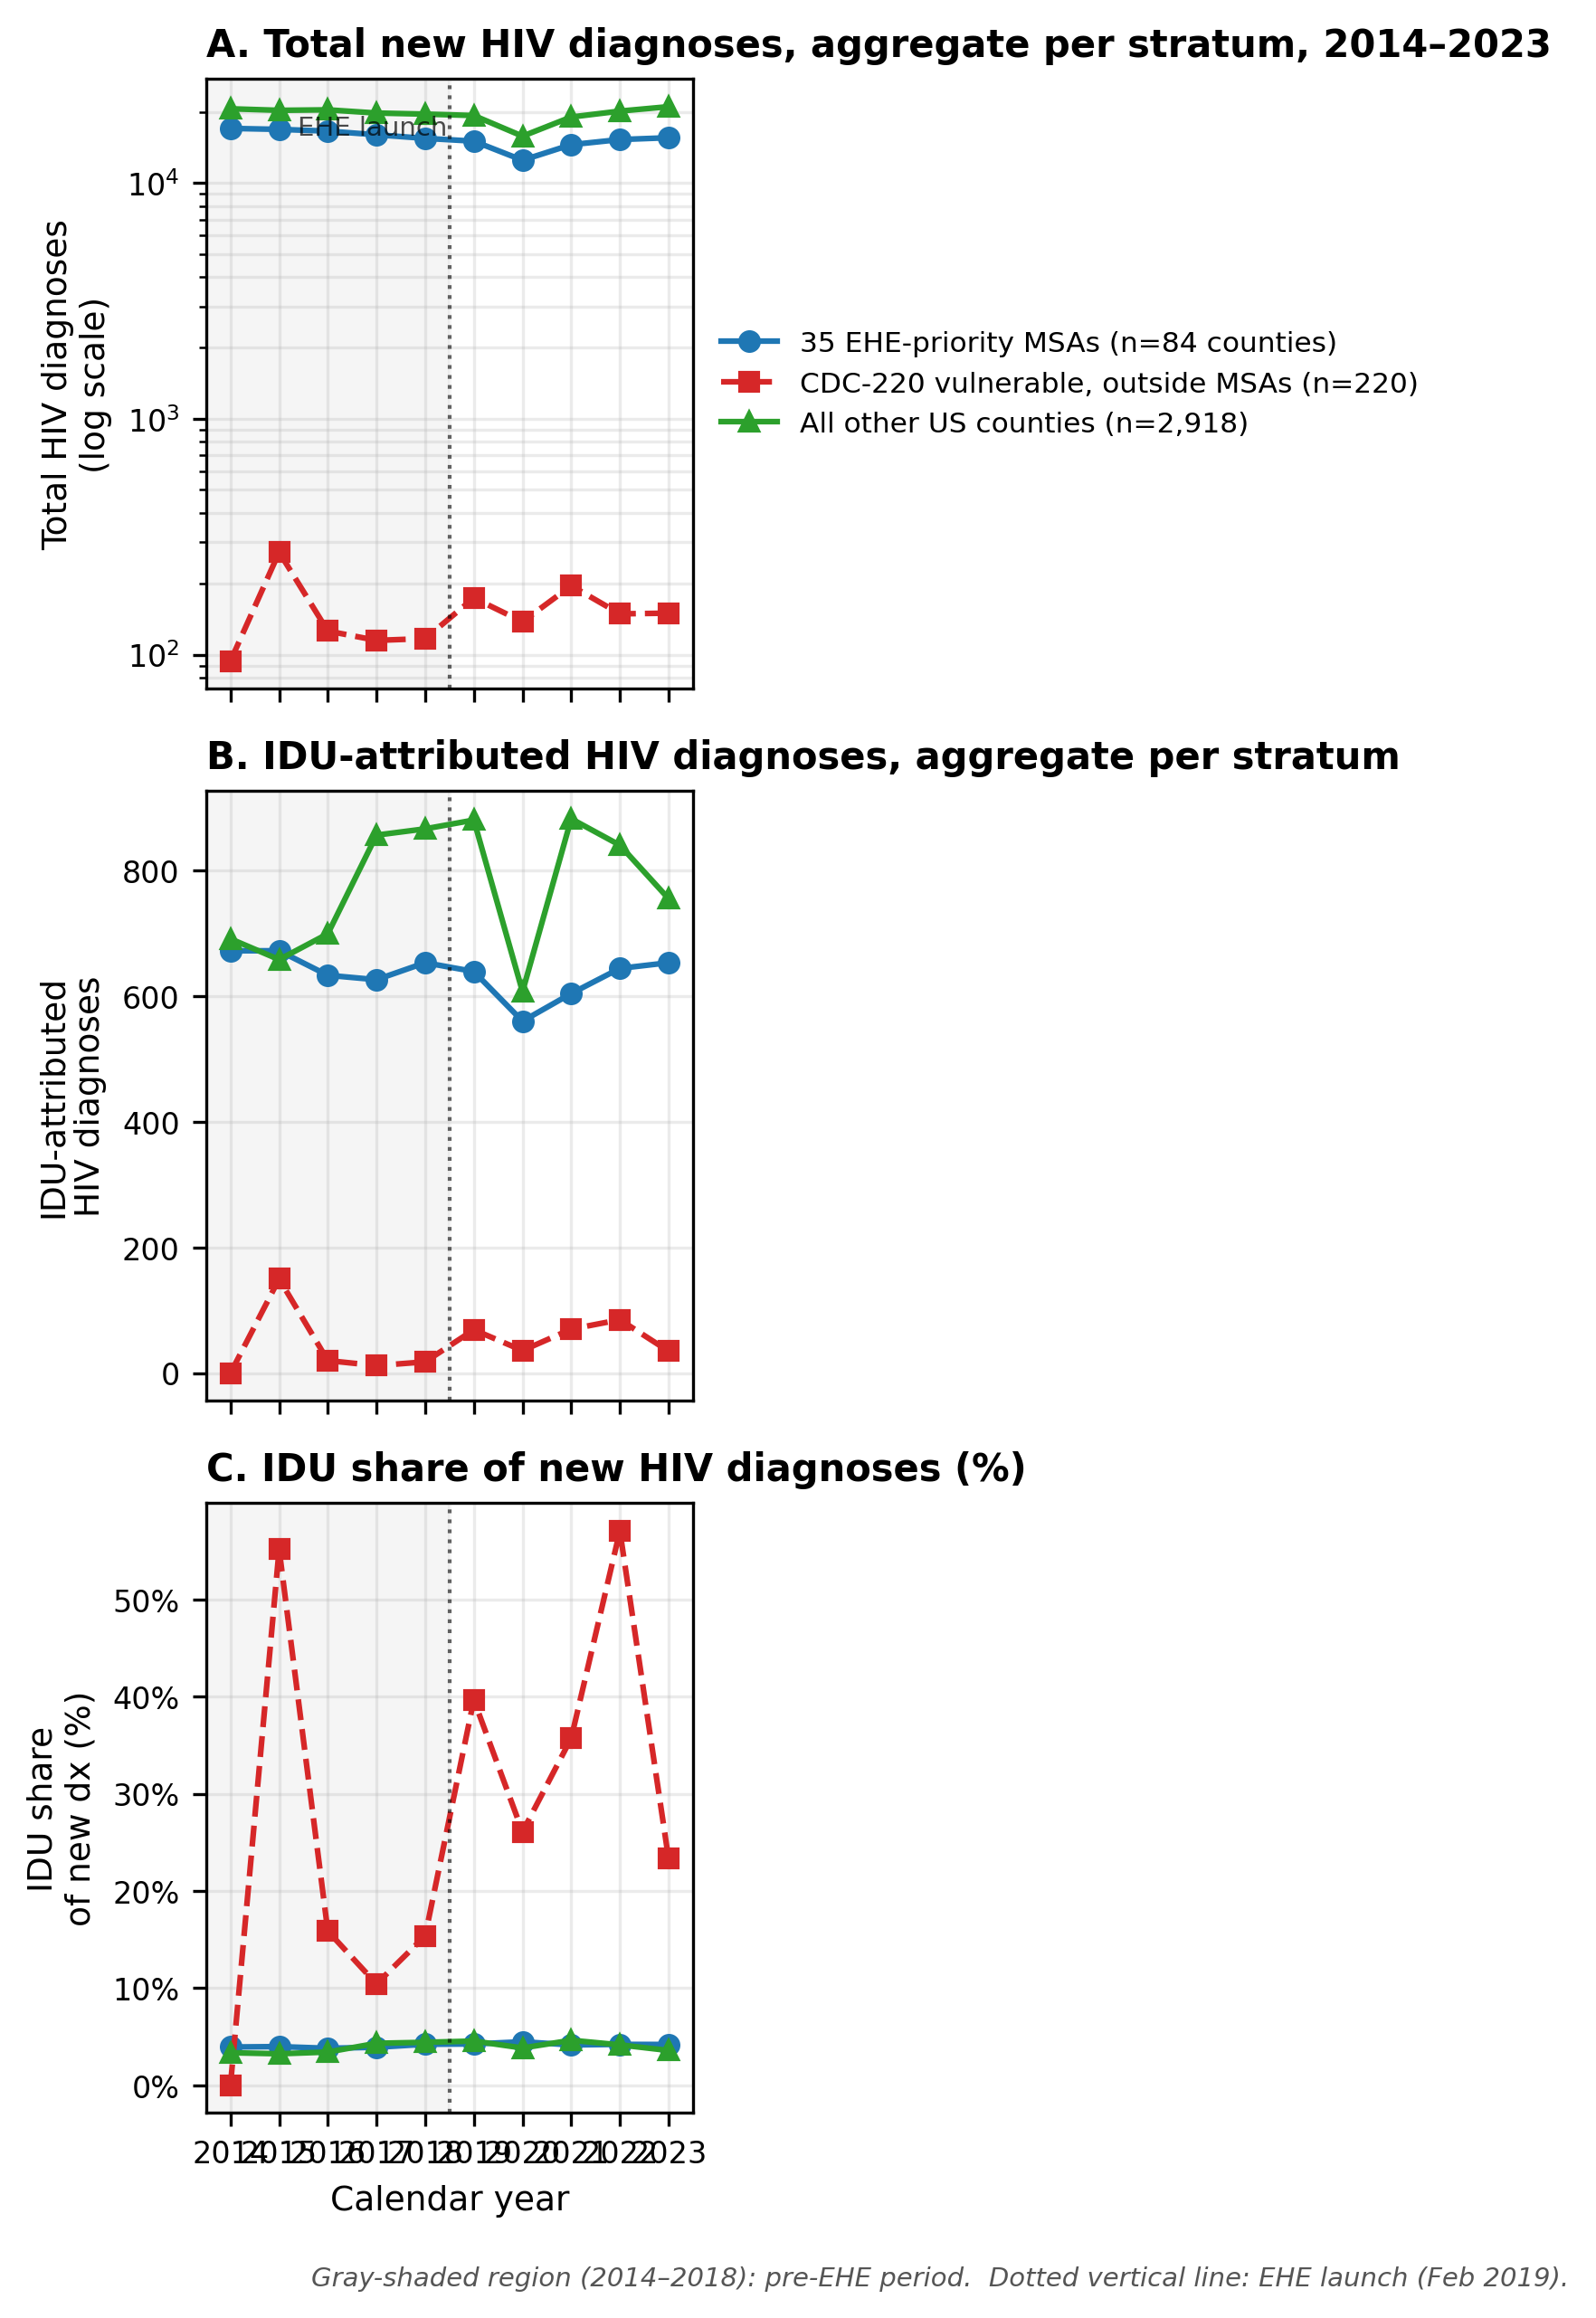
\includegraphics[width=\textwidth,height=0.75\textheight,keepaspectratio]{Fig_2_stratum_trajectories.png}
\caption{Stratum-aggregate longitudinal trajectories, 2014--2023. \textbf{Panel~A:} Total new HIV diagnoses per stratum (log scale). Stratum~A (35 EHE-priority MSAs, $n=84$ counties), Stratum~B (CDC-220 vulnerable counties outside MSAs, $n=220$), Stratum~C (all other US counties, $n \approx 2{,}918$). \textbf{Panel~B:} IDU-attributed HIV diagnoses per stratum. Stratum~C shows monotonically increasing IDU dx 2014--2023 ($+9\%$), while Strata~A and B remain stable or declining. \textbf{Panel~C:} IDU share of new diagnoses (\%). Stratum~B exhibits volatility consistent with cell-size suppression of low-count counties in the AIDSVu surveillance series. Gray-shaded region indicates the pre-EHE period (2014--2018); dotted vertical line marks EHE launch (February 2019). The geographic locus of absolute IDU diagnosis growth lies outside both the EHE-priority MSAs and the 2012--2013 CDC vulnerable-county index.}
\label{fig:stratum_trajectories}
\end{figure}

\paragraph{Kassanjee correction invariance test.} Across all 34 high-burden US MSAs in a policy-iteration Markov Decision Process derived from the cascade-blocking framework~\cite{demidont_barriers_synergy}, the optimal cascade intervention sequence $\mu^*(\cdot)$ is identical with and without the Kassanjee structural-severity correction applied (Spearman $\rho$ on value-function rankings $= 0.9979$; 34/34 cities converge on the same optimal arm; step-by-step policy-match rate 100\% across all five cascade steps). The Kassanjee correction inflates value-function magnitudes by 6.2\%--17.1\% across cities---a meaningful magnitude effect---but alters the optimal policy decision in zero MSAs. If $L$ were a noisy or arbitrary measurement-error proxy for $\gamma$, applying or removing the correction would systematically alter policy decisions in a non-trivial subset of cities. It does not. This invariance is the cleanest empirical confirmation of the structural-functions reframing: $L$ and $\gamma$ are sufficiently tightly coupled---as joint structural functions of the same latent substrate $U$---that the Kassanjee correction's information content is fully absorbed by the cascade-blocking framework itself. Figure~\ref{fig:invariance} displays the invariance scatter.

\begin{figure}[ht]
\centering
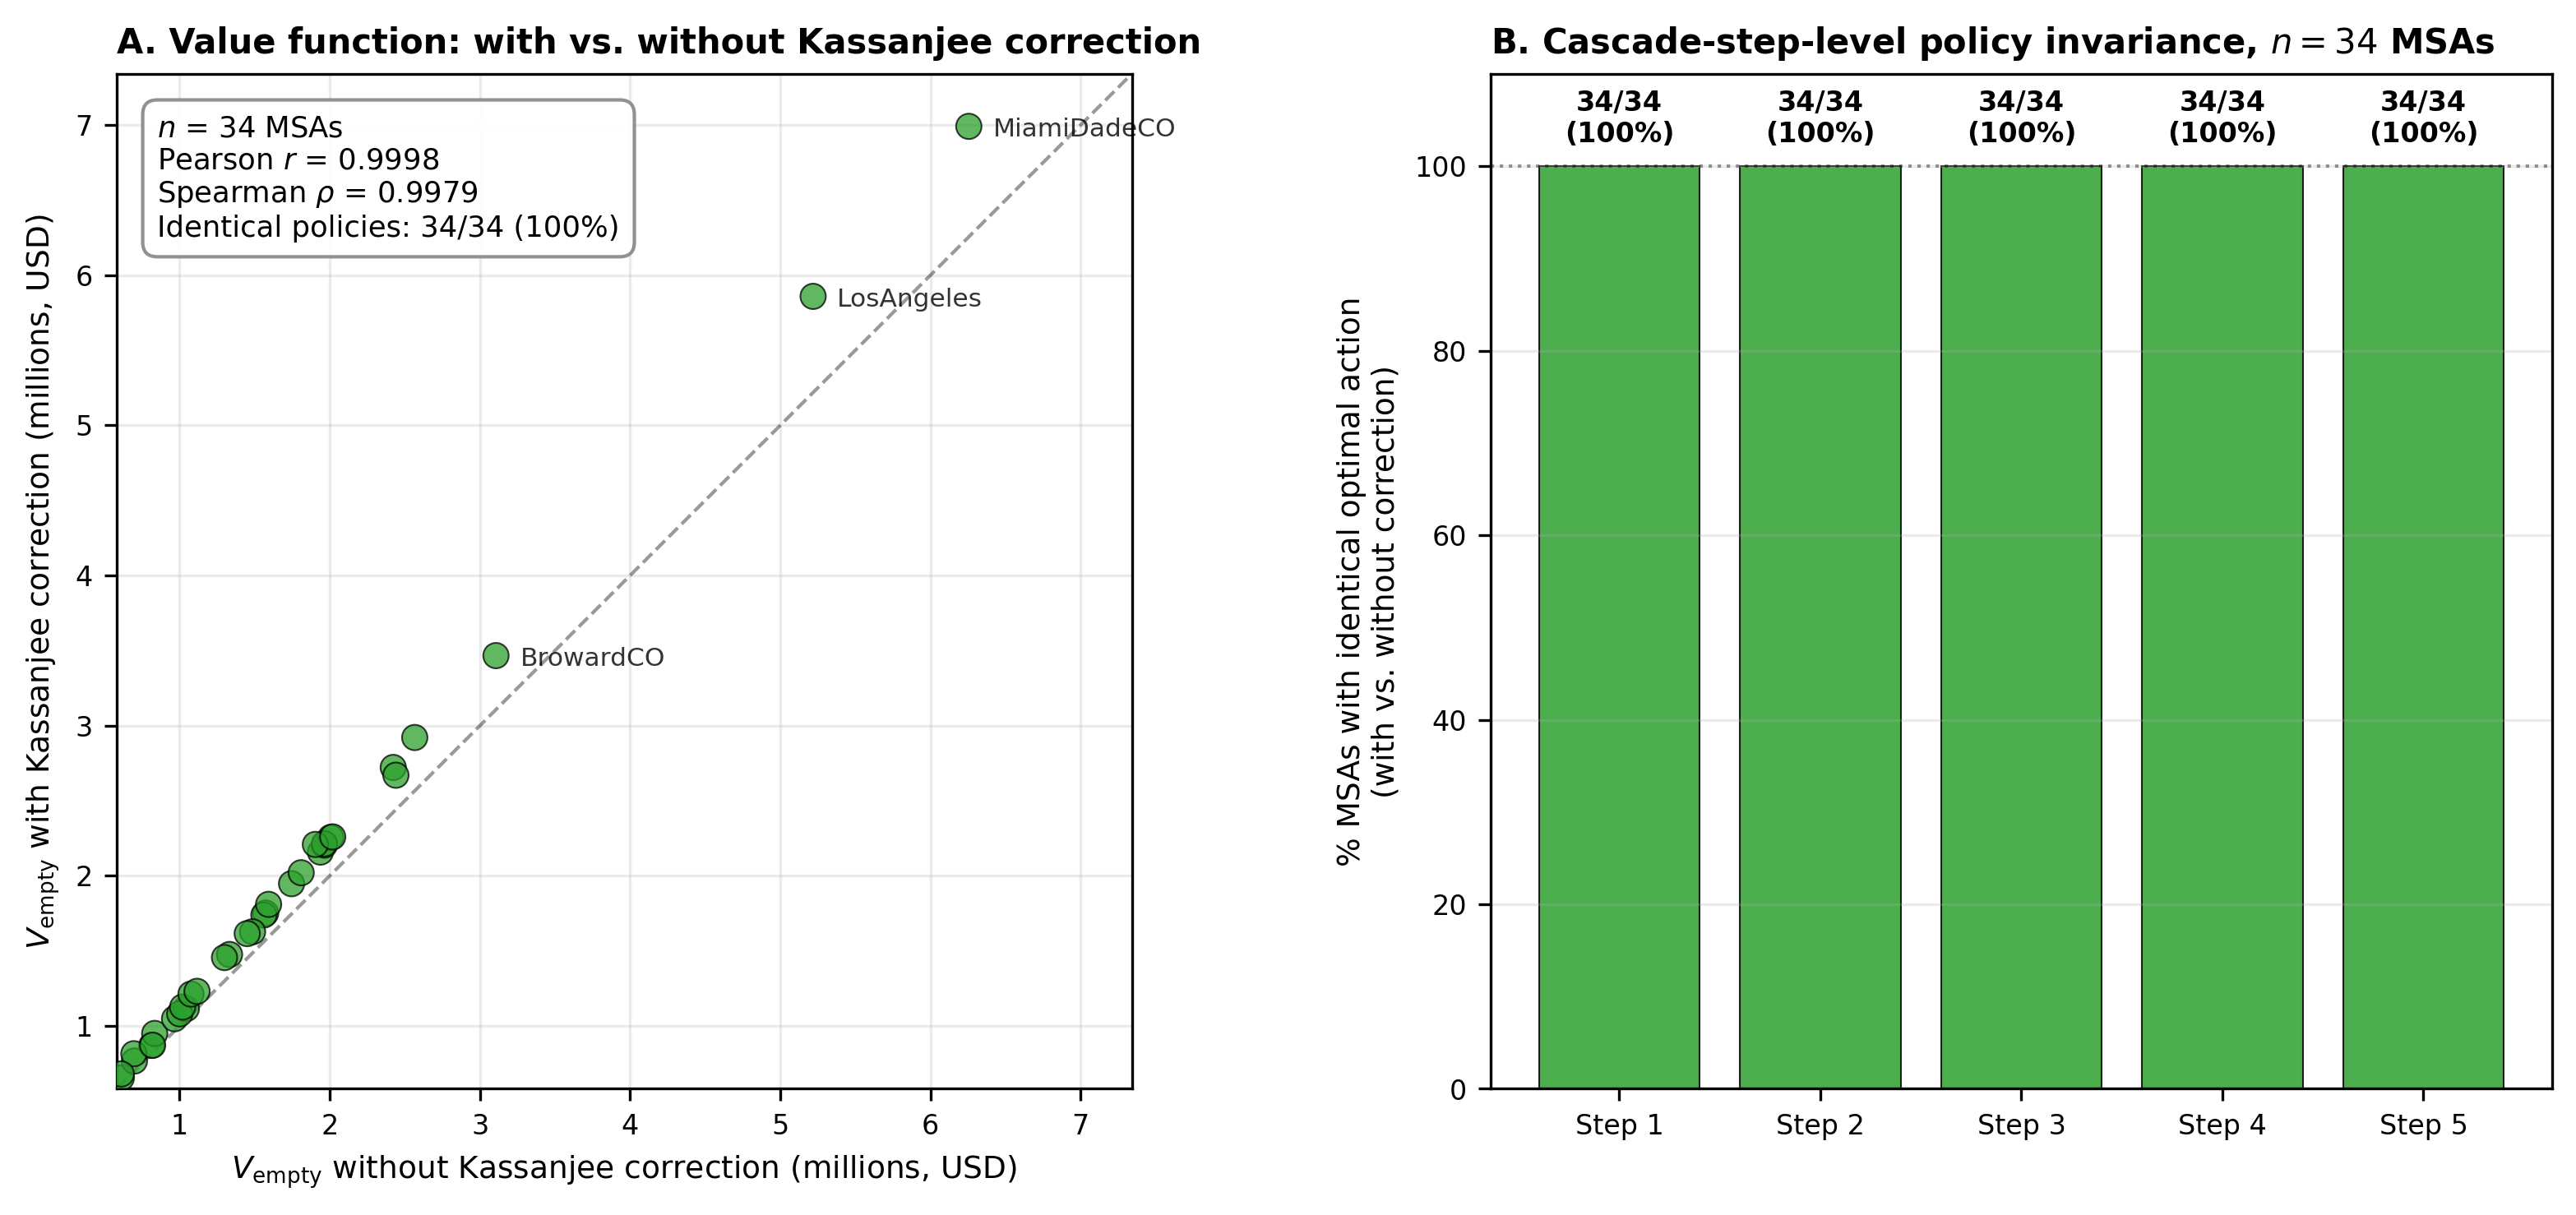
\includegraphics[width=0.95\textwidth]{Fig_3_kassanjee_invariance.png}
\caption{Kassanjee correction invariance test across 34 high-burden US MSAs. \textbf{Panel~A:} Value function (millions, USD) without Kassanjee structural-severity correction (x-axis) vs with correction (y-axis). Each point is one MSA. Dashed line is identity. Pearson $r = 0.9998$, Spearman $\rho = 0.9979$. Although the Kassanjee correction inflates value-function magnitudes by 6.2\%--17.1\% across cities (visible as systematic offset above the identity line), all 34 cities (100\%) yield identical optimal cascade policies under both parameterizations. The three labeled points (Miami-Dade Co., Los Angeles, Broward Co.) are the highest-magnitude MSAs and remain on the identity-preserving line. \textbf{Panel~B:} Step-by-step policy-match rate across the five cascade steps (SSP-prepositioning, CHW peer navigation, pharmacist-initiated PEP, telehealth 24/7, ED low-barrier kits). Every step matches at 34/34 (100\%). The invariance is uniform across cities and across cascade steps, confirming that the Kassanjee correction's information content is fully absorbed by the cascade-blocking framework parameterization.}
\label{fig:invariance}
\end{figure}

Taken together with the cross-sectional bias structure characterized in §4.2--§4.4 and the transportability framing in §4.5, the longitudinal evidence sharpens the operational concerns developed in §5.1. The structural-functions reframing is not a theoretical construct introduced to handle a reviewer concern about proxy validation; it is an empirically-anchored claim about the data-generating process whose predictions are consistent with a decade of US HIV surveillance.

\section{Implications and prospective correction}

\subsection{Operational consequences in network-clustered populations}

The bias structures derived here act on observed $b_{\mathrm{HIV}}$ (via $\Omega^*$ deflation) and on observed efficacy (via $B_{\mathrm{IRR}}$ attenuation) in the same direction in populations with elevated structural hazard: both attenuate toward apparent superiority. For coverage-planning frameworks calibrated against observed incidence to derive PrEP-coverage targets, the two biases compound. True incidence in trajectory-non-stationary populations is systematically larger than the Kassanjee-derived estimate, and the per-person efficacy used to back-calculate required coverage is systematically larger than the deployment-population value. The combined error is a coverage target set against an incidence floor that is too low and an efficacy ceiling that is too high.

The operational consequence of this compounding is determined by the joint probability of three empirically-documented convergences that co-locate in the same US subpopulations. The first convergence is testing engagement failure: trajectory-non-stationary populations exhibit low HIV testing frequency, with surveillance data indicating fewer than 2\% of HIV-negative persons who inject drugs (PWID) report PrEP use [16] and a recent systematic review documenting near-complete exclusion of PWID from the PrEP best-practice implementation evidence base [17]. This is the empirical substrate of elevated $\gamma$ formalized in the present paper. The second convergence is network density above critical threshold: the same populations exhibit injection-network connectivity sufficient to sustain outbreak propagation, driven by stimulant co-injection, housing instability, and structural displacement [18, 19]. The third convergence is empirical outbreak occurrence: HIV outbreaks among PWID in the United States during the past decade have been confined to populations exhibiting both convergences one and two. Scott County, Indiana [20, 21], the Massachusetts opioid-associated outbreak of 2015--2018 [22], the Kanawha County, West Virginia outbreak of 2019--2021 [23, 24], and the King County methamphetamine-associated expansion [25] are not geographically random. They are the populations the CDC's 220-county vulnerability assessment specifically identified as carrying both elevated testing-avoidance and elevated network-density burden [26].

The product structure is what makes the consequence operationally consequential under the framework's assumptions. For trajectory-stationary populations with low $\gamma$, low network density, and no documented historical outbreak signal, the joint probability of capsid-resistance emergence at population scale is bounded near zero regardless of the LEN deployment regime, because at least one convergence factor is small. For trajectory-non-stationary populations in the AIDSVu high-severity tail, the joint probability is bounded below by the documented historical outbreak frequency, multiplied by the fraction of those populations LEN reaches, multiplied by the fraction reached under rapid-only same-day initiation protocols. None of those factors is small. In stochastic models of branching transmission with effective reproduction number $R_{\mathrm{eff}} = R_0(1 - c\epsilon)$, where $c$ is coverage and $\epsilon$ is per-person efficacy, outbreak probability is sharply nonlinear near $R_{\mathrm{eff}} = 1$. The Kassanjee bias enters this product as the factor influencing whether the deployment-population coverage target is set high enough to push $R_{\mathrm{eff}}$ below criticality: an underestimated $b_{\mathrm{HIV}}$ is consistent with an underestimated coverage requirement, the resulting coverage gap would be expected to leave $R_{\mathrm{eff}}$ above one in the high-$\gamma$ subpopulation, and the outbreak that the empirical surveillance literature has already documented in that subpopulation could continue to occur---now under conditions in which capsid resistance may be selected at breakthrough infections occurring on a same-day-rapid-initiation protocol that cannot resolve acute HIV [33, 36].

The transportability question is therefore not whether capsid-resistant LEN failure is a population-level concern in the abstract. It is unlikely to be at the global scale, because the joint probability of the three convergences is small in most populations. The transportability question is whether capsid-resistant LEN failure is a population-level concern in the specific US subpopulations where the three convergences already empirically co-occur and where LEN is now being deployed. Within the framework's assumptions, the bias structures derived here are consistent with that concern in those populations. The surveillance literature documents that the outbreak substrate already exists in those populations [18, 19, 26], and the documented historical pattern of PWID HIV outbreaks during the past decade has been confined to populations exhibiting the structural conditions the framework characterizes as high-bias---a consistency between framework prediction and empirical surveillance pattern that we treat as the form of external validation the framework admits in the absence of independent incidence measurement. The resistance pharmacology literature documents that breakthrough infection on functional monotherapy can select N74D within weeks of exposure [33, 34]. Current CDC PEP guidance acknowledges the compressed parenteral prevention window that drives the testing-resolution gap [27], and a recent systematic review of PrEP best practices documents the near-complete exclusion of PWID from the implementation evidence base on which clinical guidelines are built [17]. What appears in the cross-sectional incidence literature as nuanced statistical correction in trajectory-stationary trial cohorts has, for the clinician initiating a long-acting injectable in a patient in Charleston or Kanawha or Boston next month, the practical character of an operational hinge between containment and uncontrolled transmission of a resistance-bearing variant in a network the estimator was never calibrated to measure. The Kassanjee bias is not a methods-paper abstraction; under the framework's assumptions it is a clinically actionable indicator of which patients warrant additional bridging coverage of the acute-detection window before initiation under the current rapid-only protocol.

The longitudinal evidence presented in \S 4.6 reinforces the operational concern developed above on two axes. First, the state-vs-MSA divergence in IDU-share trends demonstrates that PWID HIV burden is migrating from the EHE-priority MSAs---where the three convergences were historically documented (Scott County, Massachusetts, Kanawha, King County) and where LEN deployment infrastructure is most concentrated---to the non-MSA jurisdictions where neither the structural interventions nor the LEN clinical trial sites are positioned. The populations toward whom same-day rapid-only initiation is operationally targeted as an equity intervention are the same populations the longitudinal record shows are increasingly outside the geographic footprint of formal HIV prevention infrastructure. Second, the CDC vulnerable-county overlay analysis demonstrates that the 2012--2013 Van Handel index has lost predictive validity for the fentanyl-era opioid landscape, meaning that the cohort of populations \S 5.1 identifies as bearing the convergence-product risk cannot be enumerated by reference to that index alone. Identifying which populations warrant additional bridging coverage of the acute-detection window before LEN initiation requires the operationally-current surveillance signal that the structural-functions framework parameterizes from late-diagnosis percentage and the broader AIDSVu indicator set---not the geographic index that the prior decade's outbreak literature was calibrated against.

The longitudinal evidence presented in §\ref{sec:longitudinal_validation} reinforces the operational concern developed above on two axes. First, the state-vs-MSA divergence in IDU-share trends demonstrates that PWID HIV burden is migrating from the EHE-priority MSAs---where the three convergences were historically documented (Scott County, Massachusetts, Kanawha, King County) and where LEN deployment infrastructure is most concentrated---to the non-MSA jurisdictions where neither the structural interventions nor the LEN clinical trial sites are positioned. The populations toward whom same-day rapid-only initiation is operationally targeted as an equity intervention are the same populations the longitudinal record shows are increasingly outside the geographic footprint of formal HIV prevention infrastructure. Second, the CDC vulnerable-county overlay analysis demonstrates that the 2012--2013 Van Handel index has lost predictive validity for the fentanyl-era opioid landscape, meaning that the cohort of populations §5.1 identifies as bearing the convergence-product risk cannot be enumerated by reference to that index alone. Identifying which populations warrant additional bridging coverage of the acute-detection window before LEN initiation requires the operationally-current surveillance signal that the structural-functions framework parameterizes from late-diagnosis percentage and the broader AIDSVu indicator set---not the geographic index that the prior decade's outbreak literature was calibrated against.

\subsection{The 22.5-day window: detection-lag is biological, not operational}

The intervention-arm detection-lag parameter $d_{\mathrm{visit}}/2 = 22.5$ days, introduced in Eq.\ 6 as the mean infection-to-detection delay under active-phase trial testing cadence, is not solely a feature of trial design. It corresponds to the upper boundary of the HIV-1 acute-infection eclipse-to-Fiebig-II window, during which an individual may be productively infected and viremic but remain undetectable on standard rapid fourth-generation antigen/antibody testing [28]. The p24 antigen component of rapid 4G assays has shown sensitivity of 0\% for Fiebig stage I/II infection in field-accuracy systematic review [29]; emergency-department surveillance against laboratory 4G algorithms identifies acute infections as missed by point-of-care rapid testing at non-trivial rates [30, 31]. Only HIV-1 RNA NAT achieves reliable Fiebig I/II sensitivity [32]. The 22.5-day parameter therefore tracks the biological boundary at which the observation process becomes adequate to the underlying signal, not an arbitrary trial-operations choice.

This boundary is operationally consequential for current implementation guidance on long-acting injectable PrEP. The PURPOSE 1 and PURPOSE 2 trials initiated lenacapavir under a triple algorithm of rapid 4G Ag/Ab, laboratory 4G Ag/Ab, and quantitative HIV-1 RNA testing [3, 4]. The 2025 WHO implementation guidance [36] and the PrEP4U pragmatic trial (NCT07335289) [37] substitute rapid 4G testing alone, with confirmatory laboratory testing returning post-injection. PrEP4U's pre-specified secondary outcome explicitly measures the proportion of individuals in whom rapid and laboratory Ag/Ab test results are consistent, and a pre-specified other outcome measures lenacapavir resistance in seroconverters [37]. These specifications quantitatively acknowledge that the rapid-only protocol is expected to generate test-discordant initiations and resistance events at non-trivial rates.

The PURPOSE 2 trial reported two HIV acquisitions in the lenacapavir arm; both seroconverters developed the N74D capsid resistance mutation [4, 36], consistent with N74D selection observed within three weeks of lenacapavir exposure under monotherapy conditions [33]. Capsid resistance-associated mutations including M66I, N74D, Q67H, and K70H confer 6-fold to greater than 1000-fold reductions in lenacapavir susceptibility [34, 35]; some carry substantial replication-fitness costs, but the M66I and Q67H/N74D variants retain sufficient fitness for clinical relevance [34]. The bias structure derived in this paper implies that the populations most likely to harbor undetected acute infection at LEN initiation are precisely the populations with elevated $\gamma$, in whom $\Omega^*$ deflation is largest. These are the same populations toward whom same-day initiation is operationally targeted as an equity intervention [27]. The convergence is structural: the populations for whom rapid-only same-day initiation is most consequential as a barrier-removal strategy are the populations in whom the testing-protocol's resolution gap is most likely to admit acute infection at injection, the populations in whom subsequent emergent capsid resistance will be most concentrated, and the populations for whom loss of LEN as a future therapeutic option carries the heaviest opportunity cost.

Bridging strategies that cover the 22.5-day window with short-acting oral antiretrovirals during the rapid-to-confirmed testing transition are not, in this framework, a clinical convenience or a precautionary measure. They are a structural requirement for the operational regime that makes rapid-only initiation defensible, and the populations in whom bridging matters most are the populations for whom omitting it generates the highest expected resistance burden. The parallel to the Prevention Theorem formalization for HIV-1 PEP [10] is exact: both papers describe a hard biological deadline (proviral integration; rapid-test seroconversion) that current implementation guidance treats as negotiable, and both demonstrate that the cost of treating it as negotiable falls disproportionately on populations whose structural conditions make timely engagement with the standard testing protocol least achievable.

\subsection{For completed trials}

Published IRR estimates should be read as conditional on the enrolled cohort's structural hazard profile, with the understanding that transportability to deployment populations requires explicit consideration of whether the deployment population's hazard profile differs from the enrolled cohort's. For populations at the high-severity end of the AIDSVu distribution, the correction factor is non-negligible and should be reported alongside the uncorrected estimate.

\subsection{For prospective trial design}

Three recommendations follow for cross-sectional incidence cohorts in future prevention trials:

\begin{enumerate}
\item[(i)] The Statistical Analysis Plan should specify the structural hazard profile of the enrolled Incidence Phase cohort using population-level surveillance indicators available at screening---minimally, late-diagnosis percentage for the catchment population.

\item[(ii)] The primary analysis should report both the standard Kassanjee/Gao estimate and a $\Omega^*(\gamma)$-corrected estimate, with $\gamma$ estimated from the catchment population's surveillance profile. The correction does not require modifying the estimator itself; it is a post-hoc adjustment to the nominal MDRI. Variance propagation follows from the Gao 2021 delta-method formulation with an additional variance component $\sigma_\gamma^2$ entering additively under standard regularity conditions; the explicit propagation derivation appears in the Supplement.

\item[(iii)] Where eligibility criteria include a testing-interval exclusion, the SAP should explicitly acknowledge the selection mechanism and report the cohort's enrolled hazard under an assumed or empirically estimated amplification factor relative to the catchment population.
\end{enumerate}

\subsection{For regulatory interpretation}

Regulatory agencies evaluating efficacy claims from counterfactual-controlled prevention trials should consider requesting, as part of standard review, explicit documentation of the enrolled cohort's structural hazard profile and its relationship to the deployment population envisioned in the proposed label. Where these profiles differ substantially, the efficacy claim should be annotated with the appropriate Kassanjee correction factor.

\subsection{Limitations}

Four limitations warrant acknowledgment.

First, the closed-form correction in Equation 3 assumes an exponential basis for $P_R(t)$ and the screening-side observation factor in Equation 7 assumes a uniform-window basis. These are projections of the true LAg-EIA response curve onto distinct one-parameter families. They agree to first order in $\gamma\tau$ within the empirical AIDSVu range; outside this range the directional behavior of $B_{\mathrm{IRR}}$ depends on basis choice (Supplement, \S S2). Exact correction under the published Sedia calibration with a non-monotone $P_R(t)$ shape is an extension that would refine but is unlikely to overturn the empirical-range conclusions.

Second, the parameterization of $\gamma_{\mathrm{city}}$ from late-diagnosis percentage is a one-variable approximation; richer parameterizations incorporating viral suppression, linkage-to-care, and IDU prevalence as independent components are straightforward extensions and are explored in the Supplement.

Third, the assumption that $\gamma$ acts identically on recently-infected and uninfected individuals within the screening window is a first-order approximation. Differential hazard between these subpopulations would modify but not eliminate $\Omega^*$ deflation.

Fourth, the $1.5\times$ selection amplification factor is derived from plausible bimodal testing-behavior models rather than direct empirical measurement; direct estimation using participant-level testing-interval data from completed trials would refine this factor.

None of these limitations reverses the directional claim within the empirical range. The correction is conservative in all four dimensions.

\subsection{Conclusion}

The Kassanjee cross-sectional incidence estimator is a powerful and broadly adopted tool in contemporary prevention-trial epidemiology. Its validity depends on a closed-system assumption that is systematically violated in populations experiencing structural censoring, and the violation is compounded by trial-design selection mechanisms that recruit the Incidence Phase cohort specifically on the testing-engagement axis that drives the underlying hazard. The bias is quantifiable, corrigible, and can be addressed prospectively in trial design without modifying the estimator itself.  The structural-functions reframing on which the correction rests is empirically anchored against a decade of US HIV surveillance: temporal persistence (AR(1) $\phi = +0.278$, test-retest $r = 0.988$), pre-EHE vs post-EHE break-points (median $\Delta = -12.4$ cases/year), state-vs-MSA divergence in IDU-share trends, the CDC vulnerable-county overlay analysis, and the Kassanjee correction invariance across 34 MSAs (Spearman $\rho = 0.9979$) each independently support the joint-manifestation-of-$U$ framing. 

The correction matters most for the populations who can least afford to have their prevention needs misestimated---those whose structural context produces both elevated risk and elevated measurement bias. Responsible use of RITA-based incidence estimation in these populations requires explicit acknowledgment of the calibration-to-deployment mismatch and transparent reporting of corrected estimates alongside the conventional ones. The conventional practice---applying a validation-cohort $\Omega$ without correction---is no longer defensible for populations with substantially elevated structural hazard relative to the calibration set.

% =====================================================
% DECLARATIONS
% =====================================================

\section*{Author contributions}

A.C.D.: conceptualization, formal analysis, mathematical derivation, numerical computation, figure generation, manuscript drafting. Sole author.

\section*{Acknowledgments}

The author thanks the HIV prevention research community whose published work informed parameter calibration.

\section*{Funding}

No external funding was received. Work conducted under the affiliation of Nyx Dynamics LLC, of which the author is sole owner.

\section*{Competing interests}

The author reports prior employment with Gilead Sciences, Inc., from January 2020 through November 2024; all Gilead stock was fully divested by December 2024. Employment ended prior to initiation of this research. Gilead Sciences had no role in conception, analysis, interpretation, writing, or the decision to submit.

\section*{Data and code availability}

All code and data-processing scripts, including the v7 longitudinal additions (panel construction, EHE break-point, state-vs-MSA divergence, Van Handel overlay, and Kassanjee correction invariance test), are available at \url{https://github.com/Nyx-Dynamics/nyx-kassanjee-letter} (Zenodo DOI: 10.5281/zenodo.19796212 for v4; v7 DOI to be minted on re-version). The AIDSVu 2023 dataset and 2014--2023 county-level panel files are publicly available at \url{https://aidsvu.org}. No individual-level data were used.

\section*{AI tool disclosure}

Computational analyses were conducted in Python (NumPy, SciPy, Matplotlib, pandas). Large language models (Anthropic Claude) were used to support manuscript drafting and readability. All AI tools were used as assistive technologies only. The author retains full responsibility for design, analysis, interpretation, and conclusions.

% =====================================================
% REFERENCES
% =====================================================

\begin{thebibliography}{99}

\bibitem{kassanjee2012} Kassanjee R, McWalter TA, Barnighausen T, Welte A. A new general biomarker-based incidence estimator. \textit{Epidemiology}. 2012;23(5):721--728.

\bibitem{gao2021} Gao F, Glidden DV, Hughes JP, Donnell DJ. Sample size calculation for active-arm trial with counterfactual incidence based on recency assay. \textit{Stat Commun Infect Dis}. 2021;13(1):20200009.

\bibitem{bekker2024} Bekker L-G, Das M, Abdool Karim Q, et al. Twice-yearly lenacapavir or daily F/TAF for HIV prevention in cisgender women. \textit{N Engl J Med}. 2024;391(13):1179--1192.

\bibitem{kelley2025} Kelley CF, Acevedo-Quinones M, Agwu AL, et al. Twice-yearly lenacapavir for HIV prevention in men and gender-diverse persons. \textit{N Engl J Med}. 2025;392(14):1261--1276.

\bibitem{aidsvu2023} AIDSVu. Downloadable datasets for US metropolitan statistical areas. Rollins School of Public Health, Emory University. 2023. \url{https://aidsvu.org}.

\bibitem{sedia} Sedia Biosciences Corporation. HIV-1 LAg-Avidity EIA: Assay package insert and calibration documentation. Portland, OR. Current revision.

\bibitem{cdc_hiv2023} Centers for Disease Control and Prevention. Monitoring Selected National HIV Prevention and Care Objectives by Using HIV Surveillance Data---United States and 6 Dependent Areas, 2023. \textit{HIV Surveillance Supplemental Report}. 2023.

\bibitem{cdc_nhbs2023} Centers for Disease Control and Prevention. HIV infection, risk, prevention, and testing behaviors among persons who inject drugs---National HIV Behavioral Surveillance. 2023.

\bibitem{bjs2023} Bureau of Justice Statistics. Prisoners in 2022---Statistical Tables. US Department of Justice. 2023.
\bibitem{vanhandel2016} Van Handel MM, Rose CE, Hallisey EJ, et al. County-level vulnerability assessment for rapid dissemination of HIV or HCV infections among persons who inject drugs, United States. \emph{J Acquir Immune Defic Syndr}. 2016;73(3):323--331.
\bibitem{demidont_finite} Demidont AC. The Prevention Theorem: Time-Dependent Constraints on Post-Exposure Prophylaxis for HIV. Preprints. January 2026. doi:10.20944/preprints202601.1090.v1. Under peer review at Science Advances.

\bibitem{demidont_barriers_synergy} Demidont AC. Structural Barriers, Stochastic Avoidance, and Outbreak Risk in HIV Prevention for People Who Inject Drugs. \emph{Preprints}. January 2026. doi:10.20944/preprints202601.0948.v1. Under peer review at BMC Public Health.

\bibitem{kuroki_pearl} Kuroki M, Pearl J. Measurement bias and effect restoration in causal inference. \textit{Biometrika}. 2014;101(2):423--437.

\bibitem{wang_blei} Wang Y, Blei DM. A proxy variable view of shared confounding. \textit{Proc 38th Int Conf Machine Learning (ICML)}. 2021;139:10697--10707.

\bibitem{miao_tt} Miao W, Geng Z, Tchetgen Tchetgen EJ. Identifying causal effects with proxy variables of an unmeasured confounder. \textit{Biometrika}. 2018;105(4):987--993.

\bibitem{proximal_causal} Tchetgen Tchetgen EJ, Ying A, Cui Y, Shi X, Miao W. An introduction to proximal causal learning. \textit{arXiv preprint}. 2020;arXiv:2009.10982.

\bibitem{pearl_causality} Pearl J. \textit{Causality: Models, Reasoning, and Inference}. 2nd ed. New York: Cambridge University Press; 2009.

\bibitem{baugher2025} Baugher AR, Wejnert C, Kanny D, et al. Are we ending the HIV epidemic among persons who inject drugs?: key findings from 19 US cities. \textit{AIDS}. 2025;39(12):1813--1819.

\bibitem{kamitani2024} Kamitani E, Higa DH, Crepaz N, Wichser M, Mullins MM. Identifying best practices for increasing HIV pre-exposure prophylaxis (PrEP) use and persistence in the United States: a systematic review. \textit{AIDS Behav}. 2024;28(7):2340--2349. doi:10.1007/s10461-024-04332-z.

\bibitem{strathdee2020} Strathdee SA, Kuo I, El-Bassel N, Hodder S, Smith LR, Springer SA. Preventing HIV outbreaks among people who inject drugs in the United States: plus ça change, plus ça même chose. \textit{AIDS}. 2020;34(14):1997--2005.

\bibitem{desjarlais2022} Des Jarlais DC, Feelemyer J, LaKosky P, et al. Potential disruptions of HIV prevention among people who inject drugs in NYC from the COVID-19 pandemic. \textit{Drug Alcohol Depend}. 2022;227:109505.

\bibitem{peters2016} Peters PJ, Pontones P, Hoover KW, et al. HIV infection linked to injection use of oxymorphone in Indiana, 2014--2015. \textit{N Engl J Med}. 2016;375(3):229--239.

\bibitem{gonsalves2018} Gonsalves GS, Crawford FW. Dynamics of the HIV outbreak and response in Scott County, IN, USA, 2011--15: a modelling study. \textit{Lancet HIV}. 2018;5(10):e569--e577.

\bibitem{alpren2020} Alpren C, Dawson EL, John B, et al. Opioid use fueling HIV transmission in an urban setting: an outbreak of HIV infection among people who inject drugs---Massachusetts, 2015--2018. \textit{Am J Public Health}. 2020;110(1):37--44.

\bibitem{bonacci2023} Bonacci RA, Moorman AC, Bixler D, et al. Prevention and care opportunities for people who inject drugs in an HIV outbreak---Kanawha County, West Virginia, 2019--2021. \textit{J Gen Intern Med}. 2023;38(3):828--831.

\bibitem{hershow2024} Hershow RB, Worthington N, Adams M, et al. A qualitative analysis of barriers to accessing HIV prevention services during an HIV outbreak among persons who inject drugs in West Virginia. \textit{AIDS Behav}. 2024;28(2):669--681. doi:10.1007/s10461-023-04254-2.

\bibitem{glick2018} Glick SN, Burt R, Kummer K, Tinsley J, Banta-Green CJ, Golden MR. Increasing methamphetamine injection among non-MSM who inject drugs in King County, Washington. \textit{Drug Alcohol Depend}. 2018;182:86--92.

% CDC 220-county vulnerability designation used for the overlay analysis in \S4.6
\bibitem{cdc220counties} Centers for Disease Control and Prevention. County-level vulnerability assessment for rapid dissemination of HIV or HCV infections among persons who inject drugs, United States (220 vulnerable counties; 2012--2013 index). 2016.

\bibitem{tanner2025} Tanner MR, O'Shea JG, Byrd KM, et al. Antiretroviral postexposure prophylaxis after sexual, injection drug use, or other nonoccupational exposure to HIV---CDC recommendations, United States, 2025. \textit{MMWR Recomm Rep}. 2025;74(1):1--56.

\bibitem{fiebig2003} Fiebig EW, Wright DJ, Rawal BD, et al. Dynamics of HIV viremia and antibody seroconversion in plasma donors: implications for diagnosis and staging of primary HIV infection. \textit{AIDS}. 2003;17(13):1871--1879.

\bibitem{lewis2015} Lewis JM, Macpherson P, Adams ER, Ochodo E, Sands A, Taegtmeyer M. Field accuracy of fourth-generation rapid diagnostic tests for acute HIV-1: a systematic review. \textit{AIDS}. 2015;29(18):2465--2471. doi:10.1097/QAD.0000000000000855.

\bibitem{white2018} White DAE, Giordano TP, Pasalar S, et al. Acute HIV discovered during routine HIV screening with HIV antigen-antibody combination tests in 9 US emergency departments. \textit{Ann Emerg Med}. 2018;72(1):29--40.

\bibitem{stekler2016} Stekler JD, Ure G, O'Neal JD, et al. Performance of Determine Combo and other point-of-care HIV tests among Seattle MSM. \textit{J Clin Virol}. 2016;76:8--13.

\bibitem{branson2014} Branson BM, Owen SM, Wesolowski LG, et al. Laboratory testing for the diagnosis of HIV infection: updated recommendations. Centers for Disease Control and Prevention. 2014.

\bibitem{wirden2024} Wirden M, Pouderoux C, Peytavin G, et al. Ultra-rapid selection of the N74D capsid inhibitor resistance mutation after 3 weeks on lenacapavir. \textit{J Antimicrob Chemother}. 2024;79(7):1706--1707.

\bibitem{pennetzdorfer2026} Pennetzdorfer N, et al. Lenacapavir treatment-emergent HIV-1 capsid resistance mutations are frequently associated with replication defects. \textit{Sci Transl Med}. 2026;18:eaea0947.

\bibitem{briganti2025} Briganti L, Annamalai AS, Bester SM, et al. Structural and mechanistic bases for resistance of the M66I capsid variant to lenacapavir. \textit{mBio}. 2025;16(5):e0361324.

\bibitem{who2025} World Health Organization. Guidelines on lenacapavir for HIV prevention and testing strategies for long-acting injectable pre-exposure prophylaxis. Geneva: WHO; 2025.

\bibitem{prep4u} PrEP4U: Assessing the Effectiveness of Integrated Same-Day Lenacapavir Initiation and Follow-up Choice on PrEP Persistence. ClinicalTrials.gov NCT07335289.

\end{thebibliography}

\end{document}